\documentclass[a4paper,11pt,leqno]{article} \usepackage{amsmath}
\usepackage{amsfonts} \usepackage{amsthm} \usepackage{amssymb}
%\usepackage{slashbox} \usepackage{tikz-cd}
\usepackage{mathrsfs} \DeclareMathAlphabet{\mathpzc}{OT1}{pzc}{m}{it}
\usepackage{graphicx} \usepackage{hyperref}
%\DeclareGraphicsExtensions{.png,.jpeg} \usepackage[bottom=1.5in, left=1.25in,
%right=1.25in, top=1.5in]{geometry}
\usepackage[bottom=1in, left=1in, right=1in, top=0.9in]{geometry}
%\usepackage{fancyhdr}
\usepackage{mathtools} \usepackage{color} \usepackage{enumitem}
\usepackage{amsthm} \usepackage{tikz}
\usetikzlibrary{decorations.markings,arrows}
%\usepackage{pgfplots} \usepackage{fancyvrb} \usepackage{linalgjh}
\usepackage{subcaption}

\DeclarePairedDelimiter{\floor}{\lfloor}{\rfloor}
%\pagestyle{fancy}
\renewcommand{\d}{\ensuremath{\operatorname{d}}}
\newcommand*{\Comb}[2]{{}^{#1}C_{#2}}% \newcommand{\sub}{\subseteq}
\newcommand{\lto}{\leftarrow} \newcommand{\inj}{\xhookrightarrow{}}
\newcommand{\NN}{\mathbb{N}} \newcommand{\ZZ}{\mathbb{Z}}
\newcommand{\CC}{\mathbb{C}} \newcommand{\ZP}{\mathbb{Z}_p}
\newcommand{\RR}{\mathbb{R}} \newcommand{\QQ}{\mathbb{Q}}
\newcommand{\FF}{\mathbb{F}} \newcommand{\curA}{\mathscr{A}}
\newcommand{\curB}{\mathscr{B}} \newcommand{\curC}{\mathscr{C}}
\newcommand{\curD}{\mathscr{D}} \newcommand{\curI}{\mathscr{I}}
\newcommand{\curM}{\mathscr{M}} \newcommand{\of}{\circ}
\newcommand{\sub}{\subseteq} \newcommand{\XOR}{\otimes}
\newcommand{\car}[1]{\overline{\overline{#1}}}
\renewcommand{\Re}{\ensuremath{\operatorname{Re}}}
\renewcommand{\Im}{\ensuremath{\operatorname{Im}}}
\newcommand{\id}{\ensuremath{\operatorname{id}}}
\newcommand{\im}{\ensuremath{\operatorname{im}}}
\newcommand{\Hom}{\ensuremath{\operatorname{Hom}}}
\newcommand{\Ext}{\ensuremath{\operatorname{Ext}}}
\newcommand{\ev}{\ensuremath{\operatorname{ev}}}
\newcommand{\Obj}{\ensuremath{\operatorname{Obj}}} \newtheorem*{thm}{Theorem}
\newtheorem*{lemma}{Lemma} \newtheorem{prop}{Proposition}
\theoremstyle{definition} \newtheorem{defn}{Definition}
\newcommand{\divides}{\bigm|} \newcommand{\notdivides}{% \mathrel{\mkern.5mu
  % small adjustment
  % superimpose \nmid to \big|
    \ooalign{\hidewidth$\big|$\hidewidth\cr$\nmid$\cr}% }%
    } \newcommand{\norm}[1]{\left\lVert#1\right\rVert}
    \newcommand{\Res}{\text{Res}} \newcommand{\del}{\partial}

\title{The mathematics of UMAP} \author{Adele Jackson}
%\chead{Banach space of continuous functions}
\begin{document} \thispagestyle{empty} \maketitle

\section{Introduction}

UMAP (Uniform Manifold Approximation and Projection) is a new dimension
reduction technique~\cite{McInnes18}, currently
implemented~\cite{McInnesGithub, MelvilleGithub} for both labelled and
unlabelled data.
Figure~\ref{fig_example_embedding} shows a comparison of UMAP embeddings with
the outputs of some other standard dimension reduction algorithms.
UMAP gives similarly good outputs for visualisation as t-SNE, with
a substantially better runtime (see~\cite{McInnesBenchmarking}), and may
capture more of the global structure of the data.
The current UMAP implementation also allows UMAP to be used as a preprocessing
step in a machine learning pipeline, as new data can be embedded into an
existing model.

\begin{figure}
  \centering
  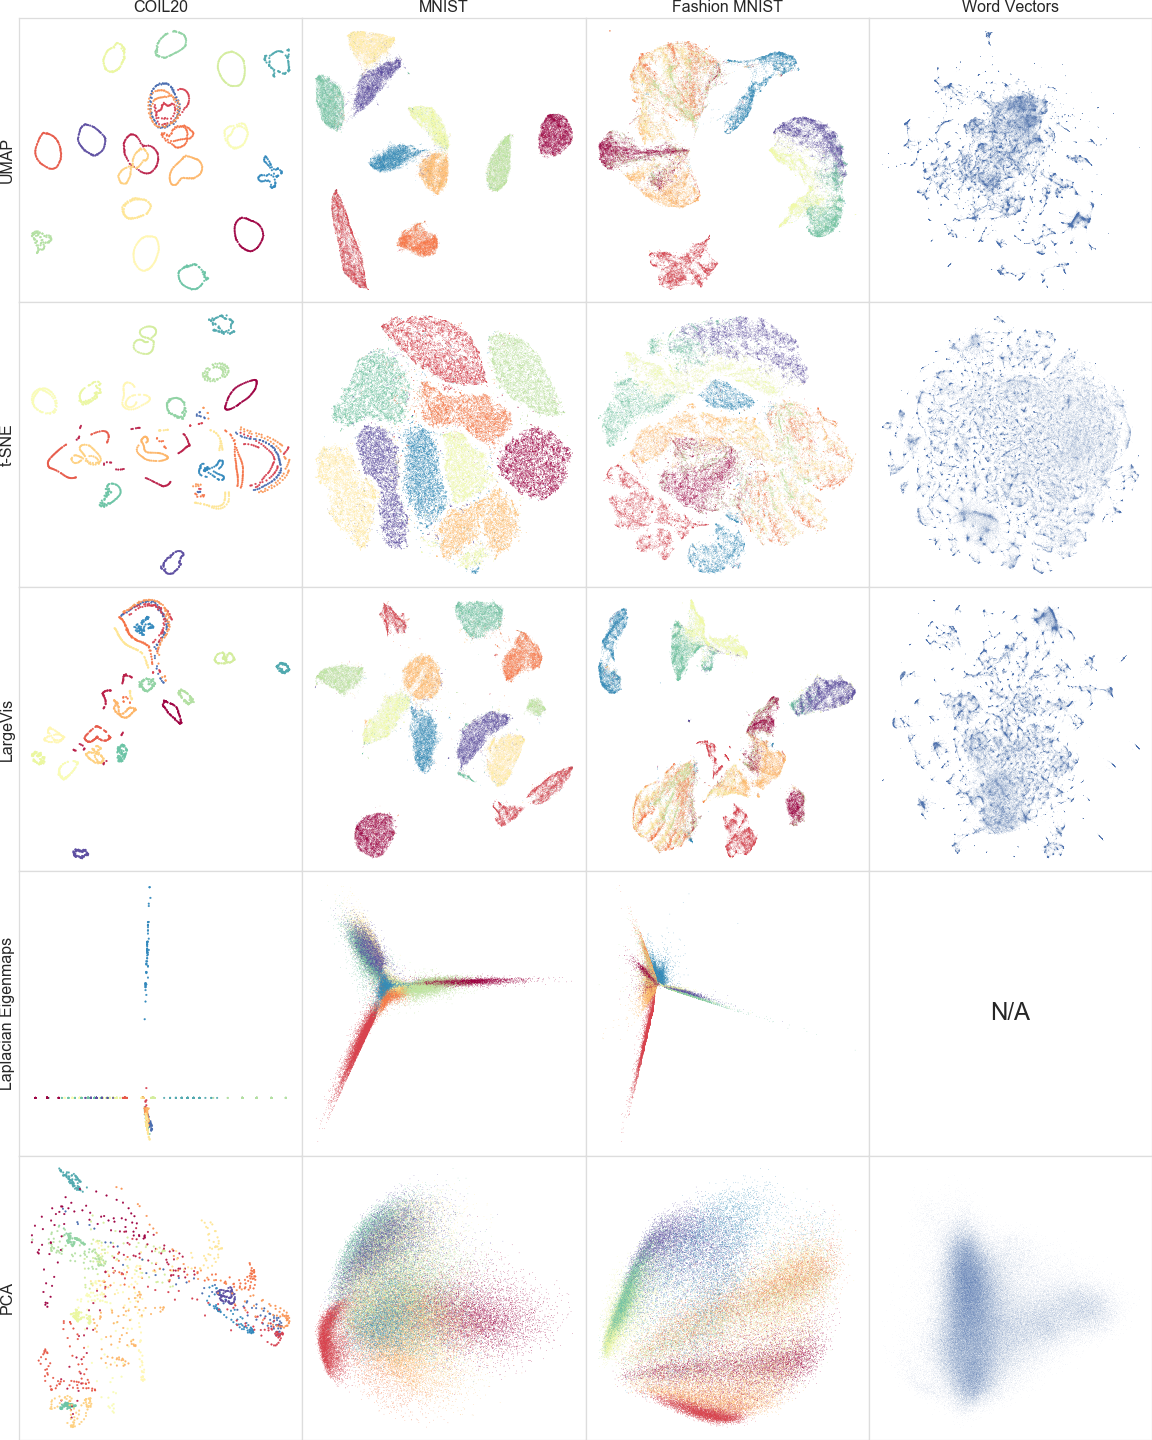
\includegraphics[width=1.05\textwidth]{figures/dim-red-comparison-nips.png}
  \caption{Embeddings from UMAP, t-SNE, LargeVis, Laplacian Eigenmaps and PCA
  on some standard datasets. Image taken from~\cite{McInnes18}.}
  \label{fig_example_embedding}
\end{figure}

Excitingly, UMAP is based on strong and general mathematical theory, which does
not depend on a Euclidean metric.
As a result, UMAP can be used for datasets with a mixture of categorical and
continuous features.

The main mathematical result behind UMAP is that there is an adjunction between
finite fuzzy simplicial sets and finite extended pseudo-metric spaces.
We will discuss what this statement means and why it is useful.
Given a dataset $D$ in $\RR^N$, we wish to find a good representation of $D$ in
a lower-dimensional space, $\RR^m$.
We wish to develop a good loss function for evaluating a lower-dimensional
representation, so we can minimise this loss.
To do this, we will construct a fuzzy simplicial set from a dataset.
A fuzzy simplicial set (which we will define in Section~\ref{section_fss}) is
an abstract description of a topological space, with probabilities on its
elements that we will interpret as giving their size.
We can then compare the fuzzy simplicial set from our dataset $D$ with that
from a proposed low-dimensional representation.

\section{Approximating the underlying manifold}
\label{section_uniform}

Given a dataset $D$ in $\RR^N$, we think of the datapoints as being drawn from
some Riemannian manifold\footnote{
  A Riemannian manifold is a space that locally looks like Euclidean space, in
  which we have well-defined notions of distances, angles, and volumes.
  For example, the surface of a unit sphere in $\RR^3$ is a two-dimensional
  Riemannian manifold.
} $M$, then mapped into $\RR^N$ by some injective map $\phi: M\to\RR^N$.
See Figure~\ref{fig_M_in_Rn} for an illustration of this setup.

One thought we might have is to reconstruct $M$, then find a good map from $M$
into $\RR^m$.  To do this, we assume that $D$ is uniformly drawn from $M$, as in
the example in Figure~\ref{fig_M_in_Rn}. (Note that parts of $M$ might be
stretched out or compressed under the map $\phi$ into $\RR^N$, so this does
{\textbf{not}} imply that the data is uniformly distributed in $\RR^N$.) This
assumption means that $D$ approximates $M$ well.  (This is also where the `U' in
UMAP comes from.) We will also assume that $M$ is locally connected and that
there are enough points in $D$ that no point in $D$ is isolated in its own
connected component.  These connectivity assumptions imply that every point in
$D$ is connected in $M$ to its nearest neighbour in $D\inj \RR^N$.  This
assumption will be used in Section~\ref{section_adjunction}.

\begin{figure}
    \centering
    \begin{subfigure}[b]{0.45\textwidth}
        $$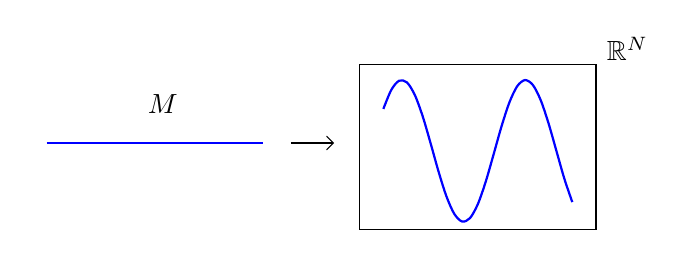
\begin{tikzpicture}
            \node (A) at (-1.1,2) {};
            \node (B) at (1.9,2) {};
            \node (C) at (0.5,2.5) {$M$};
            \node (D) at (2,2) {};
            \node (E) at (2.8,2) {};
            \node (F) at (6.4, 3.2) {$\RR^N$};
            {\path[-, thick, color=blue] (A) edge node[above]{} (B);}
            \path[->,font=\small,>=angle 90] (D) edge node[left]{} (E);
            \draw (3, 0.9) rectangle (6, 3);
            \draw plot[domain=3.3:5.7,smooth] (\x,{0.9*sin(4*\x r)+1.9})[thick, color=blue];
        \end{tikzpicture}$$
        \caption{The manifold $M$ embedded in $\RR^N$.}
    \end{subfigure}
    \begin{subfigure}[b]{0.45\textwidth}
        $$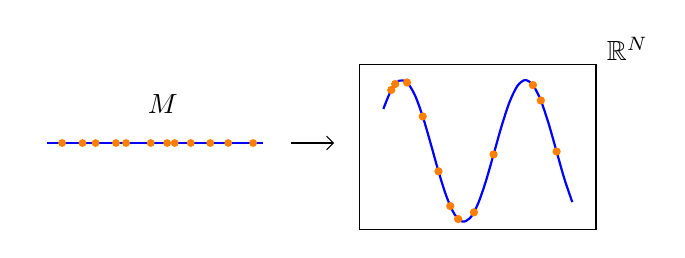
\begin{tikzpicture}
            \pgfmathsetseed{20}
            \node (A) at (-1.1,2) {};
            \node (B) at (1.9,2) {};
            \node (C) at (0.5,2.5) {$M$};
            \node (D) at (2,2) {};
            \node (E) at (2.8,2) {};
            \node (F) at (6.4, 3.2) {$\RR^N$};
            {\path[-, thick, color=blue] (A) edge node[above]{} (B);}
            \path[->,font=\small,>=angle 90] (D) edge node[left]{} (E);
            \draw (3, 0.9) rectangle (6, 3);
            \draw plot[domain=3.3:5.7,smooth] (\x,{0.9*sin(4*\x r)+1.9})[thick, color=blue];
            \foreach \i in {3.4,3.45,3.6, 3.8, 4.0, 4.15, 4.25, 4.45, 4.7, 5.2, 5.3, 5.5} {
                \fill[orange] (\i,{0.9*sin(4*\i r)+1.9}) circle (1.5pt);
            }
            \foreach \i in {1,...,12} {
                \node at (0.21428*\i-1+0.075*rand, 2)[circle,fill=orange, inner sep=1pt] {};
            }
        \end{tikzpicture}$$
        \caption{The dataset $D$ is uniformly drawn from $M$.}
    \end{subfigure}
    \begin{subfigure}[b]{0.45\textwidth}
        $$\begin{tikzpicture}
            \pgfmathsetseed{20}
            \node (A) at (-1.1,2) {};
            \node (B) at (1.9,2) {};
            \node (C) at (0.5,2.5) {$D$};
            \node (D) at (2,2) {};
            \node (E) at (2.8,2) {};
            \node (F) at (6.4, 3.2) {$\RR^N$};
            \path[->,font=\small,>=angle 90] (D) edge node[left]{} (E);
            \draw (3, 0.9) rectangle (6, 3);
            \foreach \i in {3.4,3.45,3.6, 3.8, 4.0, 4.15, 4.25, 4.45, 4.7, 5.2, 5.3, 5.5} {
                \fill[orange] (\i,{0.9*sin(4*\i r)+1.9}) circle (1.5pt);
            }
            \foreach \i in {1,...,12} {
                \node at (0.21428*\i-1+0.075*rand, 2)[circle,fill=orange, inner sep=1pt] {};
            }
        \end{tikzpicture}$$
        \caption{We see only $D$.}
    \end{subfigure}
    \caption{The dataset is drawn from a manifold embedded in $\RR^N$.}
    \label{fig_M_in_Rn}
\end{figure}

Finally, we will assume that the metric\footnote{ A \textit{metric} on a space
$X$ is a function $d: X\times X\to \RR$ such that $d(x, y) \geq 0$, $d(x, y)
= d(y, x)$, $d(x, y) = 0$ if and only if $x = y$, and $d(x, z) \leq d(x, y)
+ d(y, z)$.  We view $d(x, y)$ as the distance from $x$ to $y$.  } on $M$ is
locally constant, as this property gives us the following lemma, which will let
us approximate distances in $M$ between points in $D$ that are close enough in
$\RR^N$.  Note that, as $M$ is embedded in $\RR^N$, we can measure distance and
volume within $M$ in two ways: that of the intrinsic metric on $M$, and that of
the metric induced by $\RR^N$.

\begin{lemma}[\cite{McInnes18}] Let $(M, g)$ be a Riemannian manifold\footnote{
    In this, $M$ is the manifold and $g$ is a two-form that gives us measures of
    distance, volumes and angles.} embedded in $\RR^n$. Let $p\in M$ be a point.
  Suppose that $g$ is locally constant.\footnote{ To be precise, we assume that
  there is an open neighbourhood $U$ with $p\in U$ on which $g$ is locally
  constant, such that $g$ is a constant diagonal matrix in the ambient
  coordinates.} Let $B$ be a ball in $M$, containing $p$, whose volume is
  $\frac{\pi^{n/2}}{\Gamma(n/2+1)}$ with respect to the metric on $M$.  Then the
  distance of the shortest path in $M$ from $p$ to a point $q\in B$ is
  $\frac{1}{r}d_{\RR^n}(p, q)$, where $r$ is the radius of $B$ in $\RR^n$ and
  $d_{\RR^n}(p, q)$ is the distance from $p$ to $q$ in $\RR^n$.  \end{lemma}

Its consequence for us is that we can approximate distances around $M$ close to
our datapoints by scaling the distance in $\RR^N$.  We do this as follows.  As
we have assumed our data is uniformly distributed on $M$, any ball of a fixed
volume $R$ on $M$ should contain the same number of datapoints.  Working
backwards, let $N_k(x)$ be the ball in $\RR^N$ around a datapoint $x$ that
contains its $k$ nearest neighbours in $\RR^N$ (with respect to the distance in
$\RR^N$).  Then for any datapoint $x_i$, consider the neighbourhood of $M$ that
is sent to $N_k(x_i)$ in $\RR^N$ (that is, consider $\phi^{-1}(N_k(x_i))$).
This ball should have the same volume as if we followed the same procedure for
any other datapoint $x_j$.  By the lemma, for $k$ small enough, we can
approximate distances in $M$ from $x_i$ to one of its $k$ nearest neighbours
$x_j$ as follows.  Fix $k$ as a hyperparameter, and write $\{x_{i_1},\dots,
x_{i_k}\}$ for the $k$ nearest neighbours of $x_i$.  Then, from the lemma, we
can derive that the distance in $M$ from $x_i$ to $x_j$ is approximately
$\frac{1}{r_i}d_{\RR^N}(x_i, x_j)$, where $r_i$ is the distance to the $k^{th}$
nearest neighbour of $x_i$.  To smooth this value, and reduce the impact of
happening to have the $k^{th}$ nearest neighbour be very far away while the
$(k-1)^{th}$ nearest neighbours are clustered close to $x_i$, we take $r_i$ to
be the value such that $$\sum_{j=1}^k\exp\left(\frac{-|x_i-x_{i_j}|}{r_i}\right)
= \log_2(k).$$

This setup presents us with a problem. The distance we get from $x_i$ to $x_j$
using this method will in general be different to that from $x_j$ to $x_i$, as
$r_j\not= r_i$. We can interpret this as the fact that, while the $x_i$ are
uniformly drawn from the manifold, they are not all the same distance apart. We
need a technique for combining a family of locally-defined finite metric
spaces\footnote{ A metric space is a set of points with an associated metric.}
to get a global structure, where we have some idea of uncertainty on the metric
spaces.  For this, we will use fuzzy simplicial sets.

Note that, although we have used the $\RR^N$ metric to develop this theory, it
still holds with any other metric.  UMAP can be used with custom distance
measures and so can handle categorical data and other measures of distance
between datapoints.

At this point, we wish to set up an elegant correspondence between fuzzy
simplicial sets (combinatorial presentations of a topological space, with
probabilities on it) and finite extended-pseudo-metric spaces (metric spaces
where we allow infinite distances). To do this, we need to define the classes of
objects involved, and introduce a little category theory.

\section{Categories, functors and adjunctions}

Category theory is a branch of mathematics that unifies common concepts across
different parts of mathematics.  For example, one can take the product of two
vector spaces, or the product of two sets, or two groups.  Using ideas from
category theory, we can give one unified definition of a ``product'' and prove
results about it that are valid in all these contexts.

For the purposes of UMAP, category theory gives us an adjunction between fuzzy
simplicial sets and finite extended-pseudo-metric spaces.  An adjunction is
a translation between different domains of discourse -- for example, there is an
adjunction between sets and vector spaces that we will discuss later in the
section.  We will now define some fundamental category theory
concepts.\footnote{ See~\cite{Spivak18} for a more detailed exposition of this
material aimed at scientists.  We follow~\cite{Riehl} for these definitions.}

A \emph{category} $\curC$ is a collection of \emph{objects}, $\Obj(\curC)$, and
between each $X, Y\in\Obj(\curC)$, a collection of \emph{morphisms}
$\Hom_{\curC}(X, Y)$, satisfying the following conditions.  We write $f: X\to Y$
to mean $f\in \Hom_{\curC}(X, Y)$.  First, we can \emph{compose} morphisms: if
$f: X\to Y$ and $g: Y\to Z$, there is a specified composite morphism $gf: X\to
Z$.  Second, we have \emph{identity morphisms}: for each object $X$, there is
a specified {identity} morphism $1_X \in \Hom_{\curC}(X, X)$ (that is, $1_X:
X\to X$).  Third, the identity morphisms act as the identity under composition:
for any $f: X\to Y$, $1_Yf = f1_X = f$.  Finally, composition is
\emph{associative}: let $f: X\to Y$, $g: Y\to Z$ and $h: Z\to W$ be morphisms.
Then $h(gf) = (hg)f$.

Two familiar examples of categories are $\textbf{Vect}$, whose objects are real
vector spaces and morphisms are linear maps, and $\textbf{Set}$, whose objects
are sets and morphisms are functions between sets.

Given a category $\curC$, we can define the opposite category $\curC^{op}$,
which we will use in the next section.  This is the category whose objects are
$\Obj(\curC)$, and whose morphisms are defined by $\Hom_{\curC^{op}}(X, Y)
= \Hom_{\curC}(Y, X)$, with composition given by $g^{op}f^{op} = (fg)^{op}$.
That is, for each morphisms $f: X\to Y$ in $\curC$, there is an opposite
morphism $f^{op}: Y\to X$ in $\curC^{op}$.  (Note that these opposite morphisms
are formal maps, and there is in general not an answer to the question of where
$f^{op}$ sends some $x\in X$.  For our purposes, we will usually be taking the
opposite category where the morphisms are inclusion maps.  In this case, we
interpret the opposite morphisms as restrictions.) If we imagine each morphism
$f: X\to Y$ in $\curC$ as an arrow between its domain $X$ and codomain $Y$,
$\curC^{op}$ is the category where we ``turn all the arrows around''.

We can now define maps between categories.  A \emph{functor} between two
categories $F: \curC\to \curD$ is a map from the objects and morphisms of
$\curC$ to those of $\curD$ that sends the identity $1_X$ to $1_{F(X)}$, and
preserves composition (that is, $F(gf) = F(g)F(f)$).  For example, we can define
a functor $\textbf{Vect}\to \textbf{Set}$ taking a vector space to its
underlying set of points, and taking a linear map between vector spaces to the
induced map on the set of points.  Note that, for any category $\curC$, we have
an identity functor $1_\curC$ that is the identity on all objects and morphisms.

We can also define maps between functors themselves.  Let $\curC$ and $\curD$ be
categories, with functors $F, G: \curC\to \curD$.  A \emph{natural
transformation} $\alpha: F\to G$ is a morphism $\alpha_X: FX\to GX$ for each
$X\in \Obj(\curC)$ such that for any $f: X\to Y$ in $\curC$, $Gf\of \alpha_X
= \alpha_Y\of Ff: FX\to GY$.

We can compose natural transformations: if $F, G, H: \curC\to \curD$, with
$\alpha$ a natural transformation from $F$ to $G$ and $\beta$ one from $G$ to
$H$, then the map $\beta\alpha$ defined by $(\beta\alpha)_X = \beta_X\of
\alpha_X$ is a natural transformation from $G$ to $H$.  Thus, one can check that
the set of all functors $\curC\to\curD$ forms a category whose morphisms are the
natural transformations.

Finally, we define an adjunction.  Suppose we wish to move between two
categories $\curC$ and $\curD$, using two functors $F: \curC\to\curD$ and $G:
\curD\to\curC$.  We could ask for an equivalence of categories, which would be
if $GF = 1_{\curC}$ and $FG = 1_{\curD}$.  This is generally too strong
a requirement.  An adjunction is a weakening of the equivalence idea, and gives
a translation between two categories.  One example of an adjunction goes between
$\textbf{Vect}$ and $\textbf{Set}$ (though there is no equivalence between
them).  We have a forgetful functor $F: \textbf{Vect}\to \textbf{Set}$ that
sends a vector space to its underlying set of points.  We also have a functor
$G: \textbf{Set}\to \textbf{Vect}$ that sends a set $S$ to the free vector space
on $S$.  This is clearly not an equivalence: $FG(S)$ is the set of all finite
formal sums with real coefficients of elements of $S$.  However, $F$ and $G$
form an adjunction.

An \emph{adjunction} is a pair of functors $F: \curC\to\curD$ and $G:
\curD\to\curC$ such that there are natural transformations $\eta: 1_\curC\to GF$
and $\epsilon: FG\to 1_\curD$ satisfying some naturality conditions.\footnote{
  The naturality conditions are that for all $X\in\curC$, $1_{FX}
  = \epsilon_{FX}F\eta_X$ and for all $Y\in\curD$, $1_{GY}
  = G\epsilon_Y\eta_{GY}$.} We write $F\dashv G$ to represent this situation,
and say that $F$ and $G$ form an adjunction with $F$ the \emph{left adjoint} and
$G$ the \emph{right adjoint}.  Note that the definition is not symmetric:
$F\dashv G$ does not imply that $G\dashv F$.

\section{Fuzzy simplicial sets}
\label{section_fss}

The adjunction we will define is between fuzzy simplicial sets and extended
pseudo-metric spaces. A simplicial set is a combinatorial way of describing
a space, which generalises a simplicial complex.

A simplicial complex describes a topological space\footnote{ A topological space
is a space with associated data consisting of all open sets in the space.
Manifolds and metric spaces are topological spaces with some more structure on
them.} in a combinatorial way.\footnote{ This section follows the exposition
in~\cite{Friedman08}, which is an excellent geometrically-motivated explanation
of simplicial sets and simplicial homotopy theory. See that document for more
detail, motivation and examples of these definitions.}

A (geometric) \emph{$n$-simplex} is the convex hull spanned by a set of $n+1$
linearly independent vertices $\{x_0,\dots, x_n\}$ in Euclidean space.  That is,
a geometric $n$-simplex is $\{\sum_{i=0}^n t_ix_i\,|\, t_i\geq 0, \sum_{i=0}^n
t_i = 1\}$.  A $0$-simplex is a single point; a $1$-simplex an interval;
a $2$-simplex a triangle.  See Figure~\ref{fig_simplices} for a depiction.  Note
that the convex hull spanned by a $n$-vertex subset of the $\{x_i\}$ is itself
an $(n-1)$-dimensional simplex.  We call this a \emph{face} of the $n$-simplex.

\begin{figure} \centering
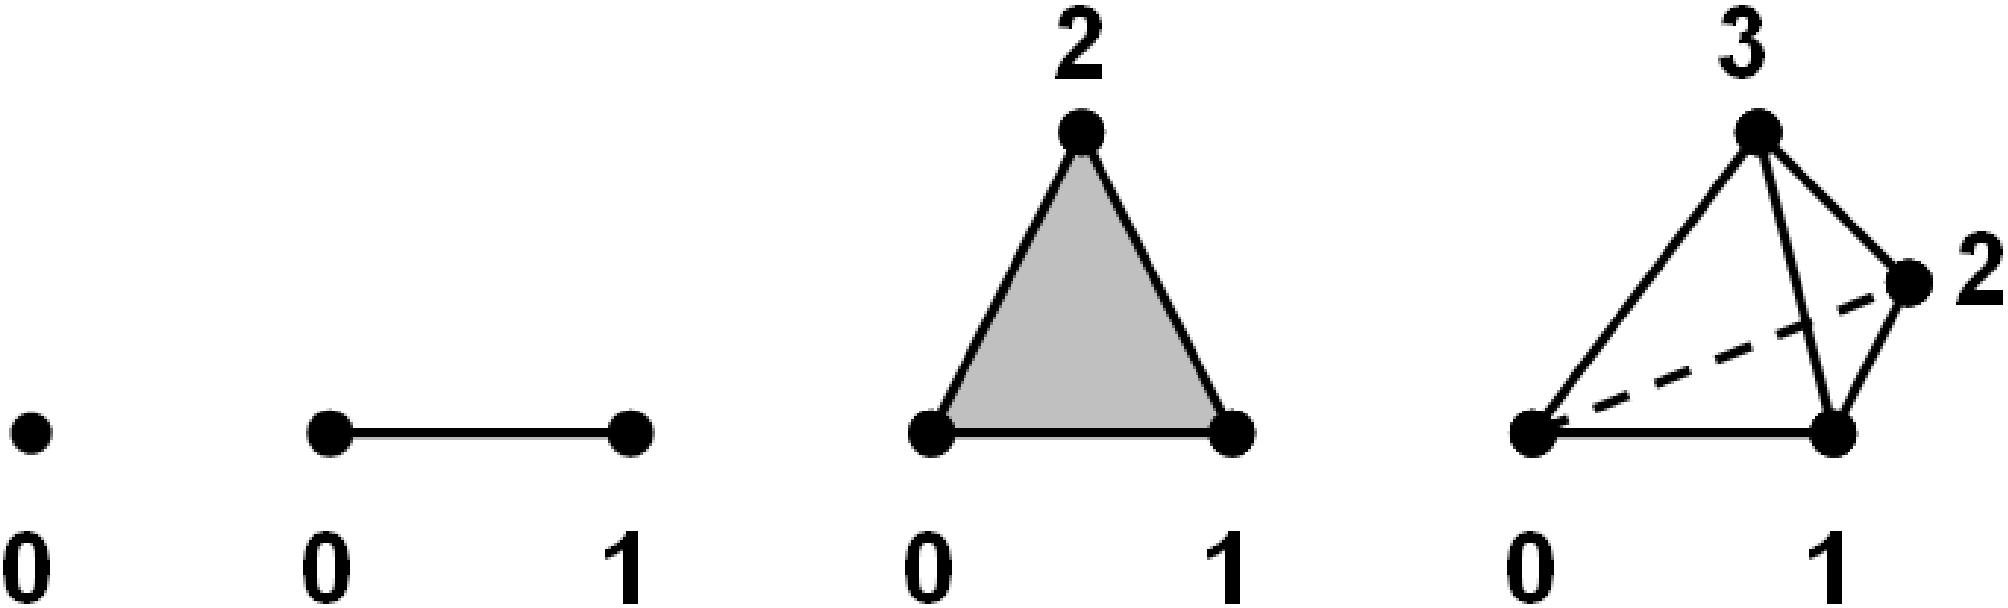
\includegraphics[width=0.7\textwidth]{figures/simp2.jpg} \caption{Examples of
$n$-simplices for $0\leq n\leq 3$. Image taken from~\cite{Friedman08}.}
\label{fig_simplices} \end{figure}

In topology, we often consider spaces up to \emph{homeomorphism}.  Let $X$ and
$Y$ be topological spaces.  A map $f: X\to Y$ is a \emph{homeomorphism} if it is
a continuous bijection with a continuous inverse.  For example, there is
a homeomorphism between a circle and an ellipse, but not between a circle and an
interval.  Note that homeomorphisms consider only the open sets of the space,
and are not affected by any metric or other structure on the space.  Geometric
$n$-simplices have the property that for any two simplices $T$ and $U$, $T$ and
$U$ are homeomorphic.

We can describe manifolds as simplicial complexes by decomposing them into
simplices.  A \emph{geometric simplicial complex} $X$ is a collection of
simplices in $\RR^N$ such that (a) for any simplex in $X$, all of its faces are
also in $X$, and (b) for any two simplices in $X$, their intersection is either
empty or is a face of both of them.  Note that, up to homeomorphism, we can
describe $X$ by listing the vertices of each simplex.  Common vertices then
allow us to recover which simplices share faces.

Generalising this idea, as simplices are defined by their vertices, an
(abstract) \emph{simplicial complex} $X$ is a series of sets $X^i$ ($i\geq 0$)
such that the elements of $X^n$ (the $n$-simplices) are $(n+1)$-element sets
that satisfy the following condition: for any $\{x_i\}_{i=0}^n\in X^n$, any
$n$-element subset of this set is in $X^{n-1}$.  Note that different simplices
can have common elements, which indicates they have vertices, edges, or other
sub-faces in common.  For example, we can describe a square $S$, formed by
gluing two triangles together, by \begin{align*} S^0	&=
\{\{a\},\{b\},\{c\},\{d\}\} & S^1	&= \{\{a, b\}, \{a, c\}, \{a, d\}, \{b, c\},
\{c, d\}\}\\ S^2	&= \{\{a,b,c\}, \{a,c,d\}\}.  \end{align*} We can describe the
simplicial complex $X$ depicted in Figure~\ref{fig_simplicial_complex} by
\begin{align*} X^0	&= \{\{v_0\}, \{v_1\}, \{v_2\}, \{v_3\}, \{v_4\},
  \{v_5\}\}\\ X^1	&= \{\{v_0, v_1\}, \{v_0, v_2\}, \{v_0, v_5\}, \{v_1, v_2\},
  \{v_2, v_3\}, \{v_2, v_4\}, \{v_2, v_5\}, \{v_3, v_4\}\}\\ X^2	&= \{\{v_0,
v_1, v_2\}, \{v_0, v_2, v_5\}, \{v_2, v_3, v_4\}\}.  \end{align*}

\begin{figure} \centering
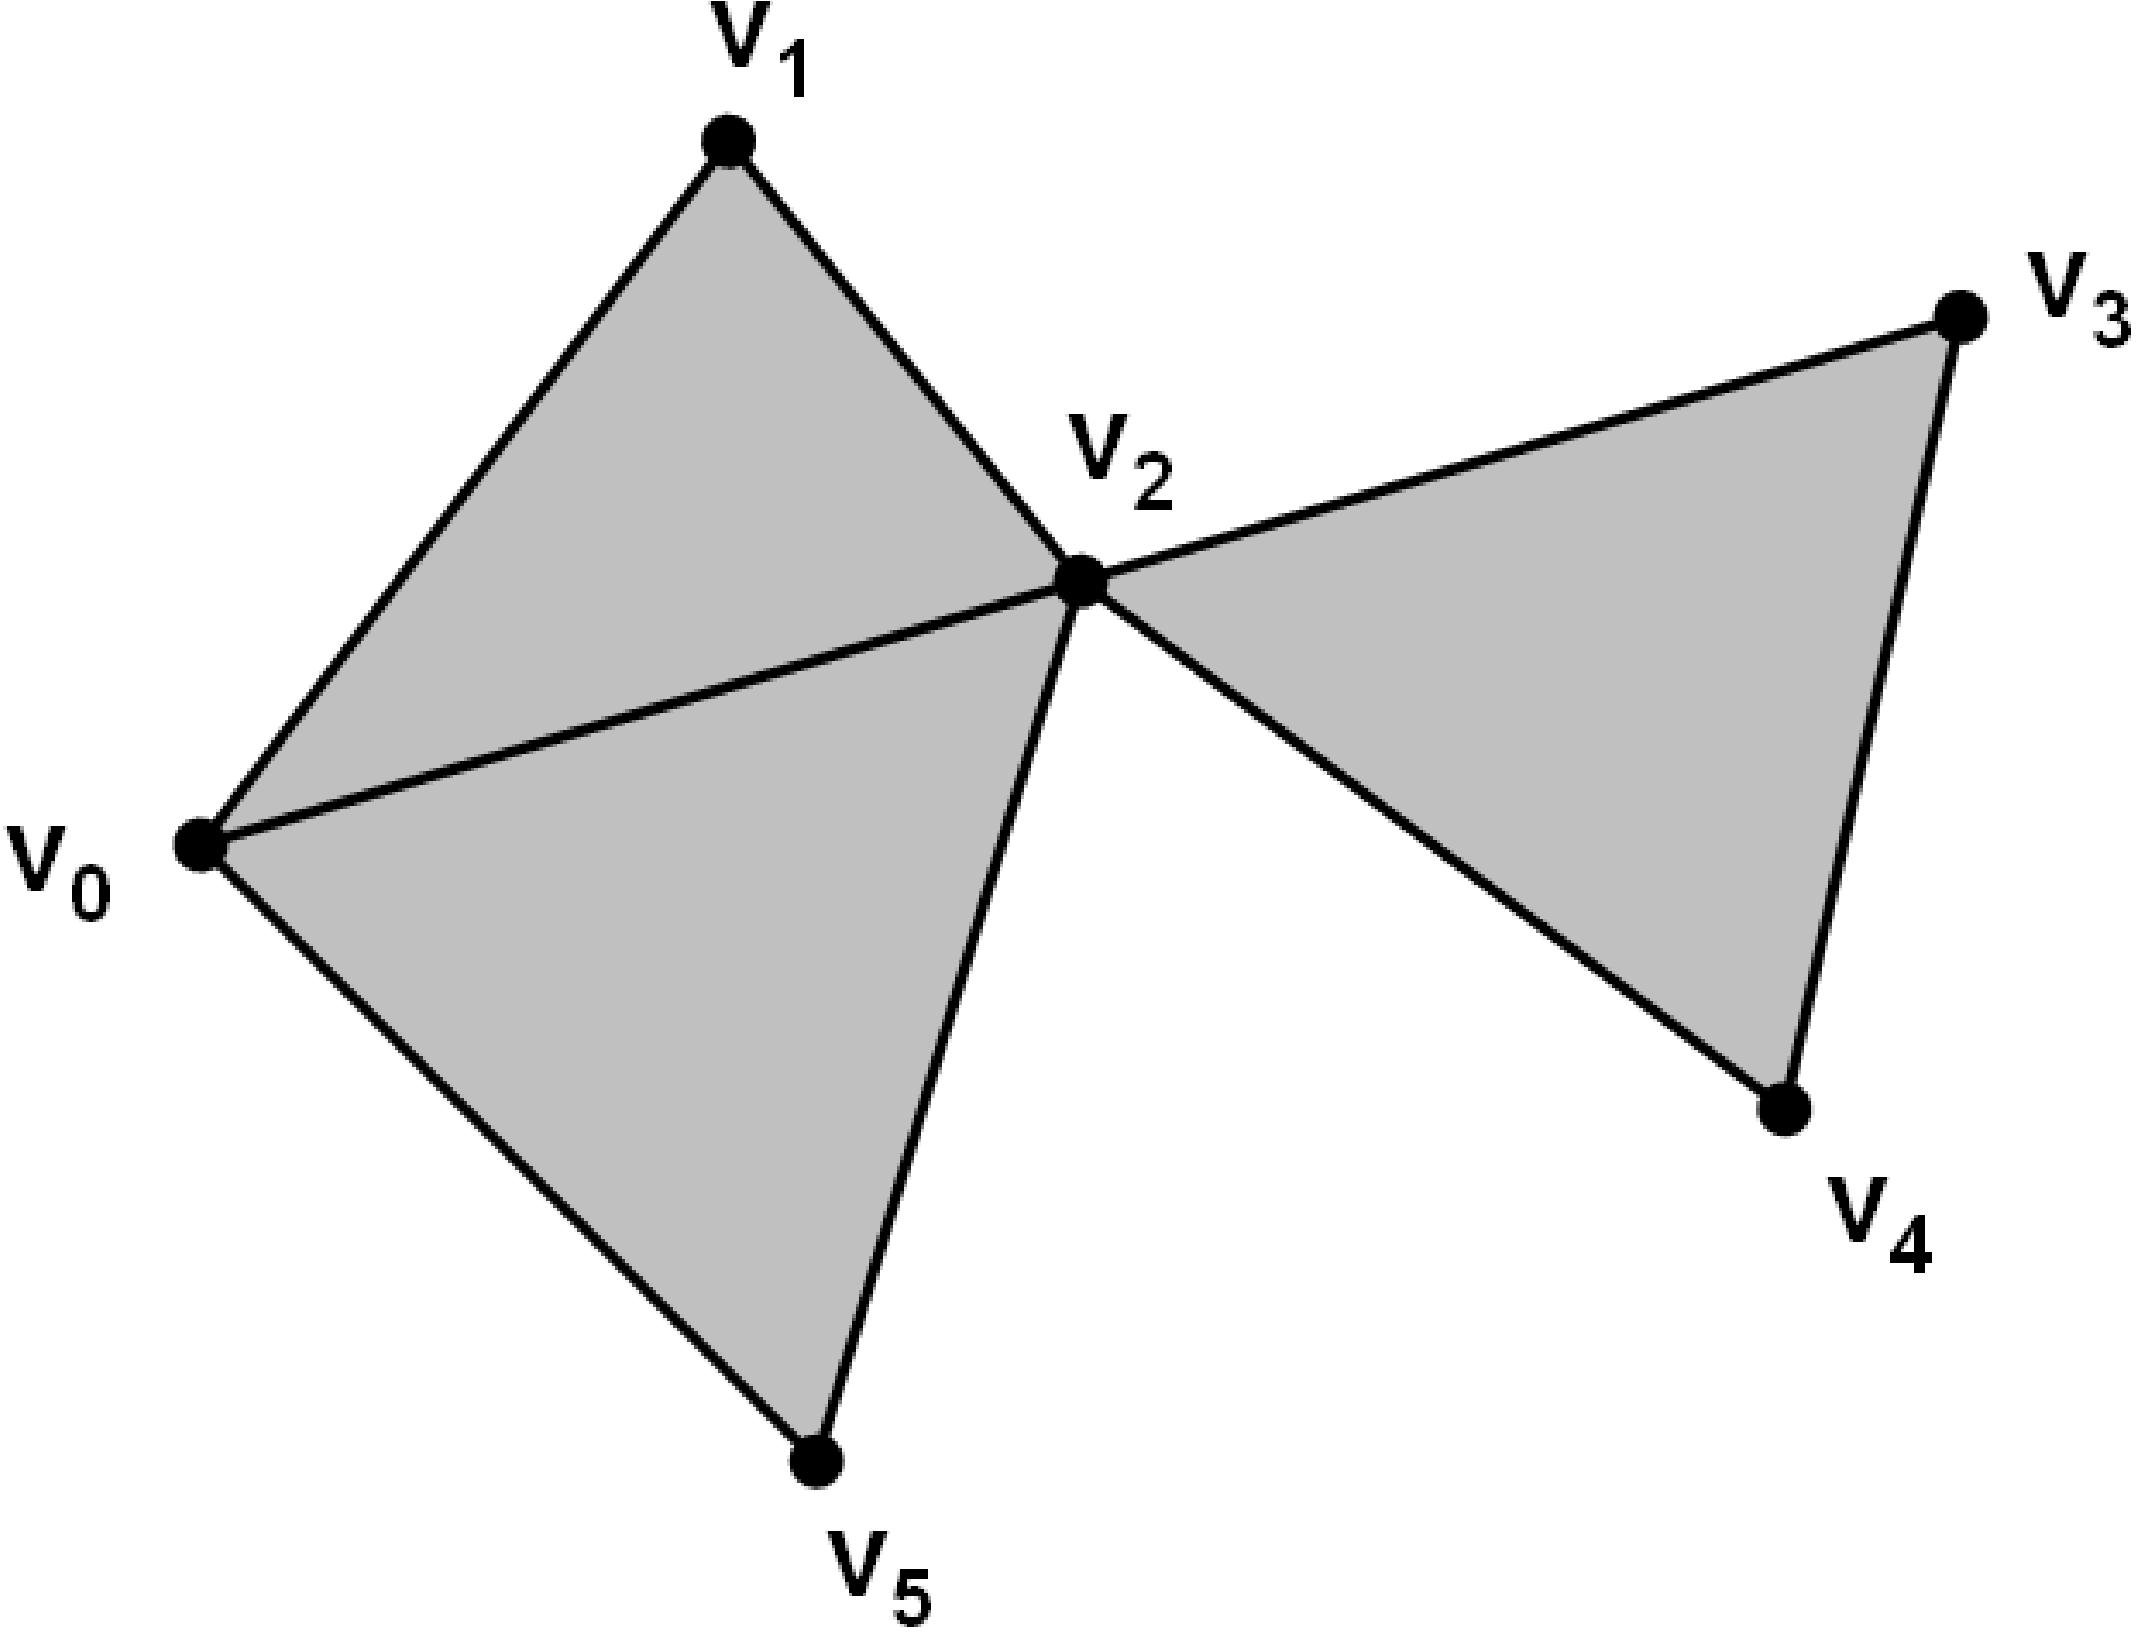
\includegraphics[width=0.4\textwidth]{figures/simp1.jpg} \caption{A simplicial
complex $X$. Image taken from~\cite{Friedman08}.} \label{fig_simplicial_complex}
\end{figure}

To abstract this idea further, let all abstract simplices come with an ordering
on its vertices.  Write an (ordered) $n$-simplex as $[x_0,\dots,x_n]$.  Note
that we can characterise an $n$-simplex in a simplicial complex by its $n+1$
\emph{face maps}, where the $i^{th}$ face map sends the simplex to the face
$[x_0,\dots, x_{i-1},x_{i+1},\dots, x_n]$; that is, it sends the simplex to the
face formed by removing the $i^{th}$ vertex from the original simplex.  Let
$d_i$ be the $i^{th}$ face map.\footnote{ Note that $d_i$ is not a map of
topological spaces. It is a formal map that to a simplex assigns its $i^{th}$
face.  Properly, we should write $d_i^n$ for the $i^{th}$ face map on
$n$-simplices. We omit the $n$ as it is almost always clear from the context.
} One can check that we have the relation that, for $i \leq j$, $d_id_j
= d_{j-1}d_i$.  Now we can give the following definition: a \emph{Delta complex}
$X$ is a collection of sets $X^i$ with, for each $n\geq 0$ and $0\leq i\leq n$,
a map $d_i: X^{n}\to X^{n-1}$ satisfying the relation $d_id_j = d_{j-1}d_i$ for
all $i\leq j$.

We interpret the elements of $X^n$ as the $n$-simplices of the Delta complex.
The difference between Delta complexes and simplicial complexes is that in
simplicial complexes, simplices are identified by their vertex set, while in
Delta complexes, two distinct simplices may share the same vertex set.  For
example, the cone depicted in Figure~\ref{fig_cone} is a Delta complex but not
a simplicial complex.

We can define Delta complexes in category theoretic language.  Let
$\hat{\Delta}$ be the category whose elements are the finite ordered sets $[n]
= [0,1,\ldots, n]$ and morphisms are strictly order-preserving maps $[m]\to
[n]$.  Then a Delta complex is a functor $X: \hat{\Delta}^{op}\to \textbf{Set}$.

We can translate between our two definitions of Delta complex as follows.  The
set $X([n])$ is the $n$-simplices of the Delta complex.  A map in
$\hat{\Delta}^{op}$ from $[n]$ to $[n-1]$, which is the opposite of an
order-preserving injection, is then a face map.  We can write maps from $[m]\to
[n]$ in $\hat{\Delta}$ as compositions of maps $[k]\to [k+1]$, so in general the
images of the morphisms under $X$ are compositions of face maps.

Now we will define a simplicial set.  Let $\Delta$ be the category whose
elements are the finite ordered sets $[n]$, and whose morphisms are
order-preserving maps $[m]\to [n]$.  (Compare to $\hat{\Delta}$ where the
morphisms are strictly order-preserving maps.) A \emph{simplicial set} is
a functor $X: \Delta^{op}\to \textbf{Set}$.

The difference between a Delta complexes and a simplicial set is that in
a simplicial set, we allow degenerate simplices.  For example, in $\Delta$,
there is a map $[0, 1, 2]\to [0, 1]$ that takes $0\mapsto 0$, $1\mapsto 1$ and
$2\mapsto 1$.  The image of this map under a simplicial set $X$ is a map $s:
X^1\to X^2$ that takes 1-simplex (an edge) $e\in X^1$ to some ``2-simplex'' in
$X^2$.  We can interpret this 2-simplex as a \emph{degenerate} 2-simplex (a
triangle) that has been collapsed into an edge.  A simplicial set carries the
information of all its degenerate simplices.

A \emph{fuzzy set} is a generalisation of a set where, rather than elements
being either in the set or not, there is a continuous membership function which
one can think of as a probability.  It is a set of objects $A$ and a function
$\mu: A\to [0, 1]$, where if $\mu(a) = 1$, $a$ is definitely in the fuzzy set.
The category $\textbf{Fuzz}$ of fuzzy sets has fuzzy sets as objects, and maps
of sets $f: A\to B$ such that $f\of \mu(a) \geq \mu(a)$ as morphisms.\footnote{
  We can also define fuzzy sets categorically. Let $I$ be the interval $[0, 1]$
  with the topology whose open sets are generated by intervals $[0, a)$.  Let
  $\curI$ be the category of open subsets of $I$ where the morphisms are
  inclusion maps.  Then a fuzzy set $S$ is a functor $S: \curI^{op}\to
  \textbf{Set}$ satisfying the following conditions. We interpret $S([0, a))$ to
  be the set of elements of $S$ of membership strength at least $a$. Let
  $\rho_{b, a}$ be the inclusion map $[0, a)\to [0, b)$ for $b\geq a$. Then $S$
  is a fuzzy set if (a) it is a sheaf and (b) the restriction maps $S(\rho_{b,
  a})$ are injections. See~\cite{Weng} for the definition of a sheaf in the
  category theoretic language we want here, where you replace the category of
  R-modules with with $\textbf{Set}$.} (That is, the maps are functions that
take elements of $A$ to elements of $B$ of the same or higher membership
strength.) Then a \emph{fuzzy simplicial set} is a functor $X: \Delta^{op}\to
\textbf{Fuzz}$.\footnote{ One nice property of these fuzzy simplicial sets is
that the membership strength of the face of a simplex is at least the membership
strength of the simplex.}

\section{Converting between metric spaces and fuzzy simplicial sets}
\label{section_adjunction}

We will now define an extended pseudo-metric space, which formalise our metric
spaces defined relative to a datapoint, and give the adjunction from
these to fuzzy simplicial sets.

Let $x_i$ be a fixed datapoint in the dataset $D$.  From
Section~\ref{section_uniform}, using the manifold metric based at $x_i$, we can
approximate the distance from $x_i$ to any other point $x_j$ in $D$ by
$d_{x_i}(x_i, x_j) = \frac{1}{r_i}d_{\RR^N}(x_i, x_j)$.  This gives us a partly
defined metric space, where we know the distance between $x_i$ and $x_j$ for all
$j$, but not between $x_j$ and $x_k$ for $j, k\not= i$.  Let $\rho_i$ be the
distance from $x_i$ to its nearest neighbour in $D$ in $\RR^N$.  As we have
assumed $M$ is locally connected, to force $x_i$ to be connected to its nearest
neighbour, for $j\not= i$, set $$d_{x_i}(x_i, x_j)
= \frac{1}{r_i}(d_{\RR^N}(x_i, x_j)-\rho_i).$$ Now, this definition means that
$x_i$ and its nearest neighbour are distance 0 apart.  As, for $j, k\not= i$, we
do not know the distances between $x_j$ and $x_k$ relative to $x_i$, we set this
to infinity.  In summary, $$d_{x_i}(x_j, x_k) = \begin{cases}
\frac{1}{r_i}(d_{\RR^N}(x_j, x_k)-\rho_i) & \text{if $j = i$ or $k = i$}\\
\infty	& \text{otherwise.} \end{cases}$$ We now no longer have a metric space:
instead we have the following generalisation.

An \emph{extended-pseudo-metric space} is a set $X$ and a function $d: X\times
X\to \RR\cup\{\infty\}$ such that (a) $d(x, y) \geq 0$, (b) $d(x, x) = 0$, (c)
$d(x, y) = d(y, x)$ and (d) either $d(x, z) = \infty$ or $d(x, z) \leq d(x, y)
+ d(y, z)$.  Note that this allows for infinite distances, and also for $d(x, y)
= 0$ when $x\not= y$.

Let $\textbf{EPMet}$ be the category of extended-pseudo-metric spaces where the
morphisms are non-expansive maps.  Let $\textbf{FinEPMet}$ be the sub-category
of $\textbf{EPMet}$ whose objects are finite extended-pseudo-metric spaces.
Note that each of our approximations of distances within $D$ is an element of
$\textbf{FinEPMet}$.

Let $\textbf{sFuzz}$ be the category of fuzzy simplicial sets (which are
functors $\Delta^{op}\to \textbf{Fuzz}$) whose morphisms are natural
transformations between the functors.  Let $\textbf{Fin-sFuzz}$ be the
sub-category of $\textbf{sFuzz}$ consisting of the fuzzy simplicial sets with
a finite number of non-degenerate simplices, defined as follows.  Let $X$ be
a fuzzy simplicial set.  An element of $X([n])$ is \emph{degenerate} if its
geometric realisation is an $(n-1)$-simplex.  The number of non-degenerate
$n$-simplices of $X$ is the number of non-degenerate elements of $X([n])$ with
positive membership strength.  Thus $X$ is in $\textbf{Fin-sFuzz}$ if it has
a finite number of non-degenerate $n$-simplices.

The main theorem of~\cite{McInnes18}, which is a slight modification of the main
theorem of~\cite{Spivak}, gives a translation between these two categories.
\begin{thm} There is an adjunction between $\textbf{FinEPMet}$ and
  $\textbf{Fin-sFuzz}$ given by $FinSing: \textbf{FinEPMet}\to
  \textbf{Fin-sFuzz}$ and $FinReal: \textbf{Fin-sFuzz}\to \textbf{FinEPMet}$,
  with $FinReal\dashv FinSing$.  \end{thm} The functors in this theorem are the
  following.\footnote{ See~\cite{McInnes18} for a categorical definition of
  these functors that makes it easier to prove they are adjoint.} The functor
  $FinReal: \textbf{Fin-sFuzz}\to\textbf{FinEPMet}$ takes a finite simplicial
  set $X$ to the finite metric space $T$ whose elements are the vertices of $X$.
  The metric on $T$ is defined as follows.  Let $\mu$ be the membership strength
  function for the simplices of $X$.\footnote{ We do not define this precisely.
  See the remark after Definition 1.1 of~\cite{Spivak} for a rigorous
  definition; Spivak's characteristic form is our membership strength function.}
  For $x, y\in T$, let $A$ be the set of all subsets of $T$ containing both $x$
  and $y$.  Then $d_T(x, y) = \min_{U\in A} -\log(\mu(U))$.

The functor $FinSing: \textbf{FinEPMet}\to \textbf{Fin-sFuzz}$ takes an finite
extended-pseudo-metric space $Y$ to a finite fuzzy simplicial set, which is
a functor from $\Delta^{op}\to \textbf{Fuzz}$.  It acts as follows:
$FinSing(Y)([n])$ is the fuzzy set of $(n+1)$-vertex subsets of the datapoints
$\{x_{k_0},\ldots,x_{k_n}\}$ where the subset has membership strength
$$\mu(\{x_{k_0},\ldots,x_{k_n}\} = \min_{i, j} e^{-d(x_{k_i}, x_{k_j})}.$$

Given this translation, we can convert a set of datapoints $D$ to a family of
elements of $\textbf{FinEPMet}$, and from that to a family of finite fuzzy
simplicial sets $FinSing(D, d_{x_i})$ for $x_i\in D$.  Now, set the \emph{fuzzy
topological representation} of $D$ to be $$\bigcup_{i=1}^n FinSing(D, d_{x_i})$$
where the union is some choice of a union of fuzzy sets.  We know that each of
the $FinSing(D, d_{x_i})$ has the same set of objects, which are all simplices
whose vertices are in $D$.  Now, if $(A, \mu)$ and $(A, \nu)$ are two fuzzy sets
with the same underlying set of objects, one reasonable definition of the union
$(A, \mu) \cup (A, \nu)$ is $(A, (\mu\cup\nu))$ where $(\mu\cup\nu)(a) = \mu(a)
\bot \nu(a)$ for $\bot$ some t-conorm.  The current implementation of UMAP uses
$x\bot y = x+y-xy$, which is the obvious t-conorm to use if you interpret
$\mu(a)$ and $\nu(a)$ as probabilities of the simplex $a$ existing, assume these
are independent between the different local metric spaces, and do not care about
higher-dimensional simplices (as, for reasons of computational complexity, we
will not).

\section{Finding a good low-dimensional representation}

We now have a method for constructing a fuzzy simplicial set from a given set of
points in $\RR^n$.  Let the dataset $D$ be in $\RR^N$.  Let $E$ be
a low-dimensional representation of our dataset $D$ in $\RR^m$, for $m < N$.  To
evaluate how good $E$ is as a representation of $D$, we compare the fuzzy
simplicial set $X$ constructed from $D$ to one constructed from $E$.  In
constructing a fuzzy simplicial set $Y$ from $E$, note that we already know the
metric of the underlying manifold as it is $\RR^m$ itself.  Thus, $Y
= FinSing((E, d))$ where $d$ is the Euclidean metric on $\RR^m$. 

Consider the sets of edges in $X$ and $Y$ as fuzzy sets.  Note that they have
the same underlying set of elements, which is all edges whose vertices are
labelled by elements of $D$, and differ only in the membership strength of the
simplices.  We define the cross-entropy $C$ of two fuzzy sets with the same
underlying elements set, $(A, \mu)$ and $(A, \nu)$, as follows~\cite[Definition
10]{McInnes18}: $$C((A, \mu), (A, \nu)) = \sum_{a\in
A}\left(\mu(a)\log\left(\frac{\mu(a)}{\nu(a)}\right)
+ (1-\mu(a))\log\left(\frac{1-\mu(a)}{1-\nu(a)}\right)\right).$$ Note that, in
our case, $\mu$ is fixed. We can view this formula as follows:
$\mu(a)\log\left(\frac{\mu(a)}{\nu(a)}\right)$ provides the attractive force, as
it is minimised if short edges in $D$ correspond to short edges in $E$, since
the length of the edge is small if $\nu(a)$ is large.  Then
$(1-\mu(a))\log\left(\frac{1-\mu(a)}{1-\nu(a)}\right)$ provides the repulsive
force, as it is minimised if long edges in $D$ correspond to long edges in $E$.
We can then optimise the embedding using stochastic gradient descent.  Note that
$X$ and $Y$ contain many simplices of high dimension.  For reasons of
computational cost, the current implementation of UMAP only looks at the
cross-entropy of the one-dimensional simplices in $X$ and $Y$. 

\section{Further reading}

The paper presenting UMAP,~\cite{McInnes18}, gives a good explanation of the
algorithm and implementation separate from its mathematical foundations.

For a geometrically-motivated definition of simplicial sets, and the realization
and singular functors in the classical (non-fuzzy) context,
see~\cite{Friedman08}.

For an introduction to category theory aimed at non-mathematicians,
see~\cite{Spivak18}. To better understand the material discussed here, you need
familiarity with adjunctions (Definition 3.70).

Spivak's proof of the adjunction between the realization and singular functors
in the fuzzy set context in~\cite{Spivak} is much more explicit than that in the
UMAP paper. Both assume familiarity with adjunctions.

\begin{thebibliography}{99}

  \bibitem{Friedman08} G. Friedman (2008). \textit{An elementary illustrated
    introduction to simplicial sets}, preprint, arXiv: 0809.4221.

  \bibitem{McInnes18} L. McInnes, J. Healy and J. Melville (2018). \textit{UMAP:
    Uniform manifold approximation and projection for dimension reduction},
    preprint, arXiv:1802.03426.

  \bibitem{McInnesVideo} L. McInnes (2018). \textit{Topological Approaches for
    Unsupervised Learning}, talk at Machine Learning Prague, accessed at
    \url{https://slideslive.com/38913519/topological-approaches-for-unsupervised-learning}.

  \bibitem{McInnesBenchmarking} L. McInnes (2018). \textit{Performance
    Comparison of Dimension Reduction Implementations}, accessed at
    \url{https://umap-learn.readthedocs.io/en/latest/benchmarking.html}.

  \bibitem{McInnesGithub} L. McInnes (2019). \textit{UMAP: Uniform manifold
    approximation and projection}, accessed at
    \url{https://github.com/lmcinnes/umap}.

  \bibitem{Melville} J. Melville (2018). \textit{UMAP Examples}, accessed at
    \url{https://jlmelville.github.io/uwot/umap-examples.html}.

  \bibitem{MelvilleGithub} J. Melville (2019). \textit{UWOT: An R package
    implementing the UMAP dimensionality reduction method}, accessed at
    \url{https://github.com/jlmelville/uwot}.

  \bibitem{Riehl} E. Riehl (2014). \textit{Category Theory in Context}, accessed
    at \url{http://www.math.jhu.edu/~eriehl/context.pdf}.

  \bibitem{Spivak18} B. Fong and D. Spivak (2018). \textit{Seven Sketches in
    Compositionality: An Invitation to Applied Category Theory}, accessed at
    \url{http:// math.mit.edu/~dspivak/teaching/sp18/7Sketches.pdf}.

  \bibitem{Spivak} D. Spivak. \textit{Metric realization of fuzzy simplicial
    sets}, accessed at
    \url{http://math.mit.edu/~dspivak/files/metric_realization.pdf}.

  \bibitem{Weng} D. Weng. \textit{A categorical introduction to sheaves},
    accessed at
    \url{http://www.math.uchicago.edu/~may/VIGRE/VIGRE2011/REUPapers/WengD.pdf}.

\end{thebibliography}

\end{document}
